\documentclass{standalone}
% analysis/style.tex — shared pgfplots preamble; % analysis/style.tex — shared pgfplots preamble; % analysis/style.tex — shared pgfplots preamble; \input{../style} from figures/
\usepackage[eulergreek]{sansmath}
\usepackage{pgfplots}
\usepackage{pgfplotstable}
\usepackage{xspace}

% Scheme-name macros — mirror the paper's meta/templates.tex so figure
% legends/titles/captions can write \plaintext / \sap / \emvp / \bntm /
% \tiptoe and render identically in both contexts. `\providecommand`
% lets the paper's templates.tex (loaded earlier) win when this file
% is in the paper as plots/pgfstyle.tex; in standalone artefact compiles
% these are the source of the macros.
\providecommand{\plaintext}{\textsc{Plaintext}\xspace}
\providecommand{\sap}{\textsc{SAP}\xspace}
\providecommand{\emvp}{\textsc{EMVP}\xspace}
\providecommand{\bntm}{\textsc{BNTM}\xspace}
\providecommand{\tiptoe}{\textsc{Tiptoe}\xspace}

\pgfplotsset{compat=newest}
\usepgfplotslibrary{units,colorbrewer,groupplots,fillbetween,statistics}
\usetikzlibrary{arrows.meta,backgrounds,calc,fit,shapes.geometric,positioning,patterns,shapes.misc}

% Bar charts request the colorbrewer Paired-12 cycle list directly via
% `cycle list/Paired-12` (loaded above by \usepgfplotslibrary{colorbrewer}).
% The library's `Paired-N` lists are full-colour, paper-quality, and live
% inside pgfplots so we don't ship a hand-rolled equivalent here.

\pgfplotsset{
  width=3.25in, height=2.5in,
  every axis/.append style={
    semithick,
    ymajorgrids=true,
    label style={font=\sffamily\small},
    title style={font=\sffamily\small},
  },
  % Line plots default to thick. `smooth` is NOT global — it is
  % opt-in per figure (added inside the axis options of figures 01,
  % 02, 04, 05, 06 that benefit from cubic interpolation). Putting
  % `smooth` in the global default fights pgfplots' `ybar` state
  % machine in figure 03 and `[only marks]` plots elsewhere; the
  % per-figure opt-in is cleaner than chasing local overrides.
  every axis plot/.append style={thick},
  legend style={
    draw=none,
    % Fully transparent legend container so overlap with plot title /
    % data points is visually obvious during figure tuning, rather
    % than silently masked. `fill=none` alone leaves an opaque white
    % rectangle on some pgfplots versions; pinning `fill opacity=0`
    % belt-and-braces guarantees see-through.
    fill=none,
    text opacity=1,
    anchor=south,
    at={(0.5,1)},
    font=\sffamily\small,
  },
  legend cell align=left,
  legend columns=-1,
  xtick align=outside,
  xtick pos=bottom,
  major tick length=1mm,
  tick label style={font=\sansmath\sffamily\small},
  every axis label={font=\sffamily\small},
  label style={font=\sffamily\small},
  {cycle list/Dark2},
  {cycle list/Set1},
  cycle list name=Dark2,
  cycle multiindex* list={
    Dark2\nextlist
    {solid,dashed,dotted,dashdotted,densely dashdotdotted}\nextlist
    mark list*\nextlist
  },
  /pgfplots/short line legend/.style={
    legend image code/.code={
      \draw[mark repeat=2,mark phase=2,##1]
        plot coordinates {(0cm,0cm)(0.2cm,0cm)(0.4cm,0cm)};
    }
  },
  /pgfplots/ybar legend/.style={
    /pgfplots/legend image code/.code={
      \draw[##1,/tikz/.cd,yshift=-0.25em](0cm,0cm) rectangle (4pt,6pt);
    },
  },
  /pgfplots/xbar legend/.style={
    /pgfplots/legend image code/.code={
      \draw[##1,/tikz/.cd,yshift=-0.25em](0cm,0cm) rectangle (4pt,6pt);
    },
  },
  select coords between index/.style 2 args={
    x filter/.code={
      \ifnum\coordindex<#1\def\pgfmathresult{}\fi
      \ifnum\coordindex>#2\def\pgfmathresult{}\fi
    }
  },
  discard if not/.style 2 args={
    x filter/.code={
      \edef\tempa{\thisrow{#1}}
      \edef\tempb{#2}
      \ifx\tempa\tempb
      \else
        \def\pgfmathresult{inf}
      \fi
    }
  },
}
 from figures/
\usepackage[eulergreek]{sansmath}
\usepackage{pgfplots}
\usepackage{pgfplotstable}
\usepackage{xspace}

% Scheme-name macros — mirror the paper's meta/templates.tex so figure
% legends/titles/captions can write \plaintext / \sap / \emvp / \bntm /
% \tiptoe and render identically in both contexts. `\providecommand`
% lets the paper's templates.tex (loaded earlier) win when this file
% is in the paper as plots/pgfstyle.tex; in standalone artefact compiles
% these are the source of the macros.
\providecommand{\plaintext}{\textsc{Plaintext}\xspace}
\providecommand{\sap}{\textsc{SAP}\xspace}
\providecommand{\emvp}{\textsc{EMVP}\xspace}
\providecommand{\bntm}{\textsc{BNTM}\xspace}
\providecommand{\tiptoe}{\textsc{Tiptoe}\xspace}

\pgfplotsset{compat=newest}
\usepgfplotslibrary{units,colorbrewer,groupplots,fillbetween,statistics}
\usetikzlibrary{arrows.meta,backgrounds,calc,fit,shapes.geometric,positioning,patterns,shapes.misc}

% Bar charts request the colorbrewer Paired-12 cycle list directly via
% `cycle list/Paired-12` (loaded above by \usepgfplotslibrary{colorbrewer}).
% The library's `Paired-N` lists are full-colour, paper-quality, and live
% inside pgfplots so we don't ship a hand-rolled equivalent here.

\pgfplotsset{
  width=3.25in, height=2.5in,
  every axis/.append style={
    semithick,
    ymajorgrids=true,
    label style={font=\sffamily\small},
    title style={font=\sffamily\small},
  },
  % Line plots default to thick. `smooth` is NOT global — it is
  % opt-in per figure (added inside the axis options of figures 01,
  % 02, 04, 05, 06 that benefit from cubic interpolation). Putting
  % `smooth` in the global default fights pgfplots' `ybar` state
  % machine in figure 03 and `[only marks]` plots elsewhere; the
  % per-figure opt-in is cleaner than chasing local overrides.
  every axis plot/.append style={thick},
  legend style={
    draw=none,
    % Fully transparent legend container so overlap with plot title /
    % data points is visually obvious during figure tuning, rather
    % than silently masked. `fill=none` alone leaves an opaque white
    % rectangle on some pgfplots versions; pinning `fill opacity=0`
    % belt-and-braces guarantees see-through.
    fill=none,
    text opacity=1,
    anchor=south,
    at={(0.5,1)},
    font=\sffamily\small,
  },
  legend cell align=left,
  legend columns=-1,
  xtick align=outside,
  xtick pos=bottom,
  major tick length=1mm,
  tick label style={font=\sansmath\sffamily\small},
  every axis label={font=\sffamily\small},
  label style={font=\sffamily\small},
  {cycle list/Dark2},
  {cycle list/Set1},
  cycle list name=Dark2,
  cycle multiindex* list={
    Dark2\nextlist
    {solid,dashed,dotted,dashdotted,densely dashdotdotted}\nextlist
    mark list*\nextlist
  },
  /pgfplots/short line legend/.style={
    legend image code/.code={
      \draw[mark repeat=2,mark phase=2,##1]
        plot coordinates {(0cm,0cm)(0.2cm,0cm)(0.4cm,0cm)};
    }
  },
  /pgfplots/ybar legend/.style={
    /pgfplots/legend image code/.code={
      \draw[##1,/tikz/.cd,yshift=-0.25em](0cm,0cm) rectangle (4pt,6pt);
    },
  },
  /pgfplots/xbar legend/.style={
    /pgfplots/legend image code/.code={
      \draw[##1,/tikz/.cd,yshift=-0.25em](0cm,0cm) rectangle (4pt,6pt);
    },
  },
  select coords between index/.style 2 args={
    x filter/.code={
      \ifnum\coordindex<#1\def\pgfmathresult{}\fi
      \ifnum\coordindex>#2\def\pgfmathresult{}\fi
    }
  },
  discard if not/.style 2 args={
    x filter/.code={
      \edef\tempa{\thisrow{#1}}
      \edef\tempb{#2}
      \ifx\tempa\tempb
      \else
        \def\pgfmathresult{inf}
      \fi
    }
  },
}
 from figures/
\usepackage[eulergreek]{sansmath}
\usepackage{pgfplots}
\usepackage{pgfplotstable}
\usepackage{xspace}

% Scheme-name macros — mirror the paper's meta/templates.tex so figure
% legends/titles/captions can write \plaintext / \sap / \emvp / \bntm /
% \tiptoe and render identically in both contexts. `\providecommand`
% lets the paper's templates.tex (loaded earlier) win when this file
% is in the paper as plots/pgfstyle.tex; in standalone artefact compiles
% these are the source of the macros.
\providecommand{\plaintext}{\textsc{Plaintext}\xspace}
\providecommand{\sap}{\textsc{SAP}\xspace}
\providecommand{\emvp}{\textsc{EMVP}\xspace}
\providecommand{\bntm}{\textsc{BNTM}\xspace}
\providecommand{\tiptoe}{\textsc{Tiptoe}\xspace}

\pgfplotsset{compat=newest}
\usepgfplotslibrary{units,colorbrewer,groupplots,fillbetween,statistics}
\usetikzlibrary{arrows.meta,backgrounds,calc,fit,shapes.geometric,positioning,patterns,shapes.misc}

% Bar charts request the colorbrewer Paired-12 cycle list directly via
% `cycle list/Paired-12` (loaded above by \usepgfplotslibrary{colorbrewer}).
% The library's `Paired-N` lists are full-colour, paper-quality, and live
% inside pgfplots so we don't ship a hand-rolled equivalent here.

\pgfplotsset{
  width=3.25in, height=2.5in,
  every axis/.append style={
    semithick,
    ymajorgrids=true,
    label style={font=\sffamily\small},
    title style={font=\sffamily\small},
  },
  % Line plots default to thick. `smooth` is NOT global — it is
  % opt-in per figure (added inside the axis options of figures 01,
  % 02, 04, 05, 06 that benefit from cubic interpolation). Putting
  % `smooth` in the global default fights pgfplots' `ybar` state
  % machine in figure 03 and `[only marks]` plots elsewhere; the
  % per-figure opt-in is cleaner than chasing local overrides.
  every axis plot/.append style={thick},
  legend style={
    draw=none,
    % Fully transparent legend container so overlap with plot title /
    % data points is visually obvious during figure tuning, rather
    % than silently masked. `fill=none` alone leaves an opaque white
    % rectangle on some pgfplots versions; pinning `fill opacity=0`
    % belt-and-braces guarantees see-through.
    fill=none,
    text opacity=1,
    anchor=south,
    at={(0.5,1)},
    font=\sffamily\small,
  },
  legend cell align=left,
  legend columns=-1,
  xtick align=outside,
  xtick pos=bottom,
  major tick length=1mm,
  tick label style={font=\sansmath\sffamily\small},
  every axis label={font=\sffamily\small},
  label style={font=\sffamily\small},
  {cycle list/Dark2},
  {cycle list/Set1},
  cycle list name=Dark2,
  cycle multiindex* list={
    Dark2\nextlist
    {solid,dashed,dotted,dashdotted,densely dashdotdotted}\nextlist
    mark list*\nextlist
  },
  /pgfplots/short line legend/.style={
    legend image code/.code={
      \draw[mark repeat=2,mark phase=2,##1]
        plot coordinates {(0cm,0cm)(0.2cm,0cm)(0.4cm,0cm)};
    }
  },
  /pgfplots/ybar legend/.style={
    /pgfplots/legend image code/.code={
      \draw[##1,/tikz/.cd,yshift=-0.25em](0cm,0cm) rectangle (4pt,6pt);
    },
  },
  /pgfplots/xbar legend/.style={
    /pgfplots/legend image code/.code={
      \draw[##1,/tikz/.cd,yshift=-0.25em](0cm,0cm) rectangle (4pt,6pt);
    },
  },
  select coords between index/.style 2 args={
    x filter/.code={
      \ifnum\coordindex<#1\def\pgfmathresult{}\fi
      \ifnum\coordindex>#2\def\pgfmathresult{}\fi
    }
  },
  discard if not/.style 2 args={
    x filter/.code={
      \edef\tempa{\thisrow{#1}}
      \edef\tempb{#2}
      \ifx\tempa\tempb
      \else
        \def\pgfmathresult{inf}
      \fi
    }
  },
}

\providecommand{\datadir}{../data}
\begin{document}
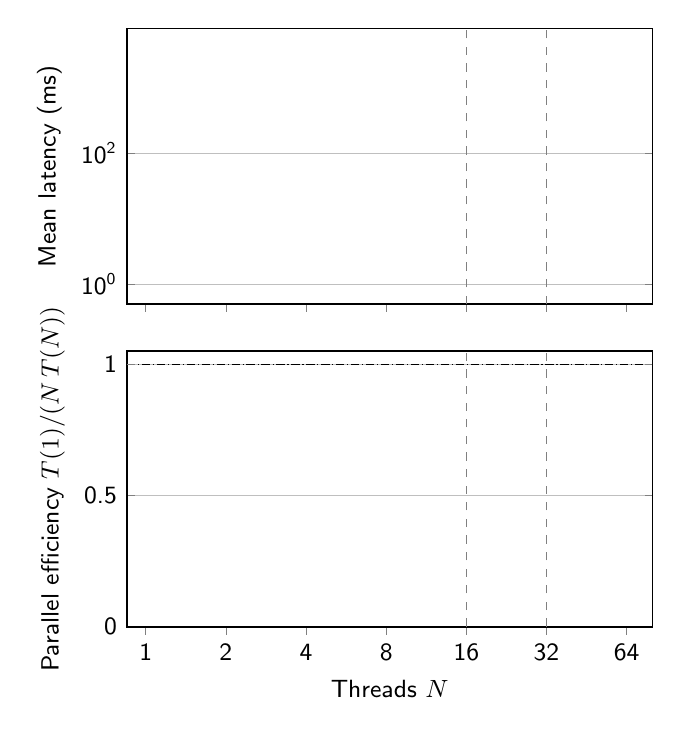
\begin{tikzpicture}
  % Per-scheme colour mapping (Dark2 palette, stable across both panels
  % and across the pinned/unpinned cut so a reader tracks one colour
  % through the whole figure). The palette index also drives the marker
  % so each scheme's identity is doubly encoded.
  \pgfplotsset{
    /pgfplots/pinned/.style   = {solid,           thick},
    /pgfplots/unpinned/.style = {dashed,          thick},
    /pgfplots/scheme1/.style  = {color=Dark2-A, mark=*},
    /pgfplots/scheme2/.style  = {color=Dark2-B, mark=square*},
    /pgfplots/scheme3/.style  = {color=Dark2-C, mark=triangle*},
    /pgfplots/scheme4/.style  = {color=Dark2-D, mark=diamond*},
    /pgfplots/scheme5/.style  = {color=Dark2-E, mark=pentagon*},
    /pgfplots/scheme6/.style  = {color=Dark2-F, mark=otimes*},
    /pgfplots/topology guide/.style = {gray, dashed, no marks, forget plot, thin},
    /pgfplots/reference/.style      = {black, densely dashdotted, no marks, forget plot, thin},
  }

  \begin{groupplot}[
    group style={
      group size=1 by 2,
      vertical sep=0.6cm,
      x descriptions at=edge bottom,
    },
    width=3.25in, height=2in,
    xmode=log, log basis x=2,
    xmin=0.85, xmax=80,
    xtick={1,2,4,8,16,32,64},
    xticklabels={1,2,4,8,16,32,64},
  ]

  % --------------------------------------------------------------------
  % Panel A: latency vs threads (log-log)
  % --------------------------------------------------------------------
  \nextgroupplot[
    ylabel={Mean latency (ms)},
    ymode=log,
    ymin=0.5, ymax=8000,
    legend style={at={(0.5,1.18)}, anchor=south, font=\sffamily\footnotesize, draw=none, fill=white, /tikz/every even column/.append style={column sep=4pt}},
    legend columns=3,
  ]

    % Topology guides: socket boundary (N=16) and SMT boundary (N=32).
    % Coordinates straddle the explicit ymin/ymax so the line spans the
    % full visible range; pgfplots clips to the axis frame.
    \addplot[topology guide] coordinates {(16, 0.5) (16, 8000)};
    \addplot[topology guide] coordinates {(32, 0.5) (32, 8000)};

    \IfFileExists{\datadir/parallel-scaling-plaintext.tsv}{
      \addplot+[scheme1, pinned, discard if not={binding}{physcpubind=0-15,membind=0}]
        table[col sep=tab, x=threads, y=latency_ms_mean]
        {\datadir/parallel-scaling-plaintext.tsv};
      \addlegendentry{\plaintext}
      \addplot+[scheme1, unpinned, discard if not={binding}{none}, forget plot]
        table[col sep=tab, x=threads, y=latency_ms_mean]
        {\datadir/parallel-scaling-plaintext.tsv};
    }{}
    \IfFileExists{\datadir/parallel-scaling-sap-ivf.tsv}{
      \addplot+[scheme2, pinned, discard if not={binding}{physcpubind=0-15,membind=0}]
        table[col sep=tab, x=threads, y=latency_ms_mean]
        {\datadir/parallel-scaling-sap-ivf.tsv};
      \addlegendentry{\sap+IVF}
      \addplot+[scheme2, unpinned, discard if not={binding}{none}, forget plot]
        table[col sep=tab, x=threads, y=latency_ms_mean]
        {\datadir/parallel-scaling-sap-ivf.tsv};
    }{}
    \IfFileExists{\datadir/parallel-scaling-emvp-ivf.tsv}{
      \addplot+[scheme3, pinned, discard if not={binding}{physcpubind=0-15,membind=0}]
        table[col sep=tab, x=threads, y=latency_ms_mean]
        {\datadir/parallel-scaling-emvp-ivf.tsv};
      \addlegendentry{\emvp+IVF}
      \addplot+[scheme3, unpinned, discard if not={binding}{none}, forget plot]
        table[col sep=tab, x=threads, y=latency_ms_mean]
        {\datadir/parallel-scaling-emvp-ivf.tsv};
    }{}
    \IfFileExists{\datadir/parallel-scaling-bntm-ivf.tsv}{
      \addplot+[scheme4, pinned, discard if not={binding}{physcpubind=0-15,membind=0}]
        table[col sep=tab, x=threads, y=latency_ms_mean]
        {\datadir/parallel-scaling-bntm-ivf.tsv};
      \addlegendentry{\bntm+IVF}
      \addplot+[scheme4, unpinned, discard if not={binding}{none}, forget plot]
        table[col sep=tab, x=threads, y=latency_ms_mean]
        {\datadir/parallel-scaling-bntm-ivf.tsv};
    }{}
    \IfFileExists{\datadir/parallel-scaling-tiptoe.tsv}{
      \addplot+[scheme5, pinned, discard if not={binding}{physcpubind=0-15,membind=0}]
        table[col sep=tab, x=threads, y=latency_ms_mean]
        {\datadir/parallel-scaling-tiptoe.tsv};
      \addlegendentry{\tiptoe}
      \addplot+[scheme5, unpinned, discard if not={binding}{none}, forget plot]
        table[col sep=tab, x=threads, y=latency_ms_mean]
        {\datadir/parallel-scaling-tiptoe.tsv};
    }{}
    \IfFileExists{\datadir/parallel-scaling-tiptoe-go.tsv}{
      \addplot+[scheme6, pinned, discard if not={binding}{physcpubind=0-15,membind=0}]
        table[col sep=tab, x=threads, y=latency_ms_mean]
        {\datadir/parallel-scaling-tiptoe-go.tsv};
      \addlegendentry{\tiptoego}
      \addplot+[scheme6, unpinned, discard if not={binding}{none}, forget plot]
        table[col sep=tab, x=threads, y=latency_ms_mean]
        {\datadir/parallel-scaling-tiptoe-go.tsv};
    }{}

  % --------------------------------------------------------------------
  % Panel B: parallel efficiency vs threads (linear y)
  % --------------------------------------------------------------------
  \nextgroupplot[
    xlabel={Threads $N$},
    ylabel={Parallel efficiency $T(1)/(N\,T(N))$},
    ymin=0, ymax=1.05,
    extra y ticks={1.0},
    extra y tick labels={},
    extra y tick style={grid=major, grid style={black, densely dashdotted, thin}},
  ]

    \addplot[topology guide] coordinates {(16, 0) (16, 1.05)};
    \addplot[topology guide] coordinates {(32, 0) (32, 1.05)};

    \IfFileExists{\datadir/parallel-scaling-plaintext.tsv}{
      \addplot+[scheme1, pinned, discard if not={binding}{physcpubind=0-15,membind=0}, forget plot]
        table[col sep=tab, x=threads, y=parallel_efficiency]
        {\datadir/parallel-scaling-plaintext.tsv};
      \addplot+[scheme1, unpinned, discard if not={binding}{none}, forget plot]
        table[col sep=tab, x=threads, y=parallel_efficiency]
        {\datadir/parallel-scaling-plaintext.tsv};
    }{}
    \IfFileExists{\datadir/parallel-scaling-sap-ivf.tsv}{
      \addplot+[scheme2, pinned, discard if not={binding}{physcpubind=0-15,membind=0}, forget plot]
        table[col sep=tab, x=threads, y=parallel_efficiency]
        {\datadir/parallel-scaling-sap-ivf.tsv};
      \addplot+[scheme2, unpinned, discard if not={binding}{none}, forget plot]
        table[col sep=tab, x=threads, y=parallel_efficiency]
        {\datadir/parallel-scaling-sap-ivf.tsv};
    }{}
    \IfFileExists{\datadir/parallel-scaling-emvp-ivf.tsv}{
      \addplot+[scheme3, pinned, discard if not={binding}{physcpubind=0-15,membind=0}, forget plot]
        table[col sep=tab, x=threads, y=parallel_efficiency]
        {\datadir/parallel-scaling-emvp-ivf.tsv};
      \addplot+[scheme3, unpinned, discard if not={binding}{none}, forget plot]
        table[col sep=tab, x=threads, y=parallel_efficiency]
        {\datadir/parallel-scaling-emvp-ivf.tsv};
    }{}
    \IfFileExists{\datadir/parallel-scaling-bntm-ivf.tsv}{
      \addplot+[scheme4, pinned, discard if not={binding}{physcpubind=0-15,membind=0}, forget plot]
        table[col sep=tab, x=threads, y=parallel_efficiency]
        {\datadir/parallel-scaling-bntm-ivf.tsv};
      \addplot+[scheme4, unpinned, discard if not={binding}{none}, forget plot]
        table[col sep=tab, x=threads, y=parallel_efficiency]
        {\datadir/parallel-scaling-bntm-ivf.tsv};
    }{}
    \IfFileExists{\datadir/parallel-scaling-tiptoe.tsv}{
      \addplot+[scheme5, pinned, discard if not={binding}{physcpubind=0-15,membind=0}, forget plot]
        table[col sep=tab, x=threads, y=parallel_efficiency]
        {\datadir/parallel-scaling-tiptoe.tsv};
      \addplot+[scheme5, unpinned, discard if not={binding}{none}, forget plot]
        table[col sep=tab, x=threads, y=parallel_efficiency]
        {\datadir/parallel-scaling-tiptoe.tsv};
    }{}
    \IfFileExists{\datadir/parallel-scaling-tiptoe-go.tsv}{
      \addplot+[scheme6, pinned, discard if not={binding}{physcpubind=0-15,membind=0}, forget plot]
        table[col sep=tab, x=threads, y=parallel_efficiency]
        {\datadir/parallel-scaling-tiptoe-go.tsv};
      \addplot+[scheme6, unpinned, discard if not={binding}{none}, forget plot]
        table[col sep=tab, x=threads, y=parallel_efficiency]
        {\datadir/parallel-scaling-tiptoe-go.tsv};
    }{}

  \end{groupplot}
\end{tikzpicture}
\end{document}
